\documentclass{beamer}
\beamertemplatenavigationsymbolsempty
\usepackage{amsmath, amssymb, hyperref, graphics}
\usepackage{graphicx}
\usepackage{tikz}
\usetikzlibrary{arrows}

\title{Graph Theory Lecture 12}
\begin{document}

\begin{frame}{The method we used to show $K_{3,3}$ isn't planar generalises:}

\begin{block}{Take any cycle $C$ in a graph $G$}
\begin{itemize}
    \item If the $G$ is planar, $C$ will be drawn as a "circle"
    \item Any other vertex or edge must lie inside or outside circle
    \item Handle possibilities case by case
\end{itemize}
\end{block}

\begin{block}{Stereographic projection:}
Don't have to treat inside/outside the circle as separate cases.
\end{block}


\begin{block}{But for a complicated graph, could still be a lot of cases...}
  Best case: graph is Hamiltonian.
  \begin{itemize}
\item Don't have to put vertices inside/outside circle
  \end{itemize}
\end{block}

\end{frame}
\begin{frame}{Another example: $K_5$ isn't planar}
    \begin{block}{Use our method with Hamiltonian cycle $ABCDEA$:}
\begin{itemize}

    \item WLOG, edge $AC$ drawn inside...
    \item Then $B$ cut off from $DE$ inside, so $BD$, $BE$ outside
    \item $BD$ cuts off $C$ from $E$ on outside, so $CE$ inside
\end{itemize}
\end{block}
\begin{block}{Only have $AD$ left, but:}
\begin{itemize}
    \item $CE$ cuts it off inside
    \item $BE$ cuts it off outside
\end{itemize}
\end{block}
\begin{block}{Therefore, $K_5$ isn't planar}

\end{block}
\end{frame}

\begin{frame}{The crossing graph packages the case by case analysis}
``Edge $e_1$ is in, so edge $e_2$ out, so edge $e_3$ in, so ...'' gets tiresome.

  \begin{block}{For this slide: $G$ a graph with Hamiltonian cycle $C$}
    \begin{itemize}
    \item Some pairs of edges in $G\setminus C$ cross if drawn inside $C$
    \item Some pairs of edges can be drawn on the same side
\end{itemize}
\end{block}
\begin{definition}
  The \emph{crossing graph} Cross($G, C)$ has:
  \begin{description}
  \item[Vertices:] the edges in $G\setminus C$
  \item[Edges] $e$ and $f$ are adjacent if they cross inside $C$
  \end{description}
  \end{definition}
\begin{theorem}[Planarity Algorithm for Hamiltonian graphs]
$G$ is planar if and only if Cross($G,C$) is bipartite
\end{theorem}

\end{frame}


\begin{frame}{Example of planarity algorithm:}
\begin{figure}
  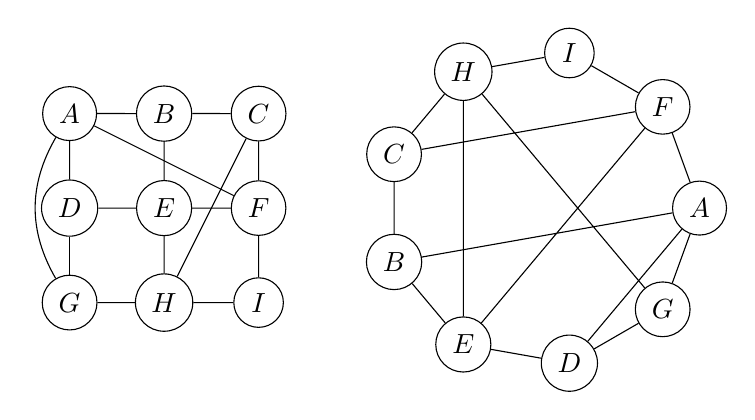
\begin{tikzpicture}[vert/.style={circle, draw}]
\begin{scope}[scale=1.2, yshift=-1cm]
  \node[vert] (A) at (0,2) {$A$};
\node[vert] (B) at (1,2) {$B$};
\node[vert] (C) at (2,2) {$C$};
\node[vert] (D) at (0,1) {$D$};
\node[vert] (E) at (1,1) {$E$};
\node[vert] (F) at (2,1) {$F$};
\node[vert] (G) at (0,0) {$G$};
\node[vert] (H) at (1,0) {$H$};
\node[vert] (I) at (2,0) {$I$};

\draw (A)--(B)--(C)--(F)--(A)--(D)--(E)--(F)--(I)--(H)--(G) to [bend left] (A);
\draw (D)--(G);
\draw (C)--(H)--(E)--(B);
\end{scope}



\begin{scope}[xshift=6cm]
  \node[vert] (A) at (0:2) {$A$};
\node[vert] (B) at (200:2) {$B$};
\node[vert] (C) at (160:2) {$C$};
\node[vert] (D) at (280:2) {$D$};
\node[vert] (E) at (240:2) {$E$};
\node[vert] (F) at (40:2) {$F$};
\node[vert] (G) at (320:2) {$G$};
\node[vert] (H) at (120:2) {$H$};
\node[vert] (I) at (80:2) {$I$};

\draw (A)--(B)--(C)--(F)--(A)--(D)--(E)--(F)--(I)--(H)--(G) to (A);
\draw (D)--(G);
\draw (C)--(H)--(E)--(B);
\end{scope}
\end{tikzpicture}
\caption{A graph $\Gamma$, then redrawn with Hamiltonian cycle outside}
\end{figure}
\begin{block}{What is Cross($\Gamma, AFIHCBEDGA$)?}
  \begin{description}
  \item[Vertices =] edges in middle
  \item[Edges =] crossings in middle
    \end{description}

\end{block}

\end{frame}
\begin{frame}{What if $G$ isn't Hamiltonian? Two lemma suffice.}

  \begin{lemma} If $G$ is a subgraph of $H$, and $G$ is nonplanar, then $H$ is nonplanar.
  \end{lemma}
  \begin{proof}
    To draw $H$, we're drawing $G$ and then adding some things.
  \end{proof}
\begin{center}
  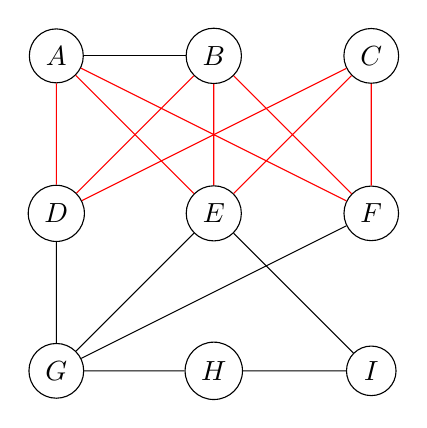
\begin{tikzpicture}[vert/.style={circle, draw}, scale=2]
\node[vert] (A) at (0,2) {$A$};
\node[vert] (B) at (1,2) {$B$};
\node[vert] (C) at (2,2) {$C$};
\node[vert] (D) at (0,1) {$D$};
\node[vert] (E) at (1,1) {$E$};
\node[vert] (F) at (2,1) {$F$};
\node[vert] (G) at (0,0) {$G$};
\node[vert] (H) at (1,0) {$H$};
\node[vert] (I) at (2,0) {$I$};


\draw[red] (F)--(A)--(D)--(B)--(E)--(C)--(F)--(B);
\draw[red] (C)--(D);
\draw[red] (A)--(E);
\draw (A)--(B);
\draw (D)--(G)--(H)--(I)--(E);
\draw (E)--(G)--(F);
\end{tikzpicture}
\end{center}
  
\end{frame}  

\begin{frame}{Another tool for showing $G$ isn't planar}        
    \begin{definition}
    A graph $H$ is a subdivision of $G$ if it can be created from $G$ by adding some vertices of degree two in the middle of edges.
    \end{definition}
    \begin{lemma}
      If $H$ is a subdivision of $G$ and, and $G$ isn't planar, then $H$ isn't planar.
    \end{lemma}
    \begin{proof} To draw $H$, we're drawing $G$ and then adding some dots on the edges.
      \end{proof}
  
\begin{center}
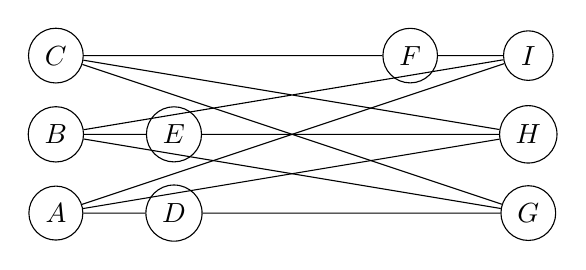
\begin{tikzpicture}[vert/.style={circle, draw}, rotate=90, yscale=3]
\node[vert] (A) at (0,2) {$A$};
\node[vert] (B) at (1,2) {$B$};
\node[vert] (C) at (2,2) {$C$};
\node[vert] (D) at (0,1.5) {$D$};
\node[vert] (E) at (1,1.5) {$E$};
\node[vert] (F) at (2,.5) {$F$};
\node[vert] (G) at (0,0) {$G$};
\node[vert] (H) at (1,0) {$H$};
\node[vert] (I) at (2,0) {$I$};
\draw (A)--(D)--(G)--(B)--(E)--(H)--(C)--(F)--(I)--(B);
\draw (H)--(A)--(I);
\draw (C)--(G);
\end{tikzpicture}
\end{center}


\end{frame}


\begin{frame}{Kuratowski's theorem -- proves a general $G$ not planar}
\begin{theorem} A graph $G$ is not planar if and only if it has a subgraph that is a subdivision of $K_{3,3}$ or $K_5$    
    \end{theorem}

\begin{block}{Proof of the ``if'' direction:}
\begin{itemize}
    \item $K_{3,3}$ and $K_5$ aren't planar
    \item So subdivisions of $K_{3,3}$ or $K_5$ aren't planar
    \item So graphs having subdivisions a $K_{3,3}$ or $K_5$
\end{itemize}
\end{block}
\begin{block}{Remarks on the ``only if'' direction}
  \begin{itemize}
  \item Harder to prove and we won't even sketch
  \item Won't \emph{explicitly} use -- if $G$ is planar, prove it by drawing it!
  \item Will use \emph{implicitly} -- if $G$ isn't planar, we know we can find a $K_{3,3}$ or $K_5$ hidden in it
    \end{itemize}
\end{block}


    
\end{frame}

\begin{frame}{Example of using Kuratowski's theorem}

  \begin{center}
  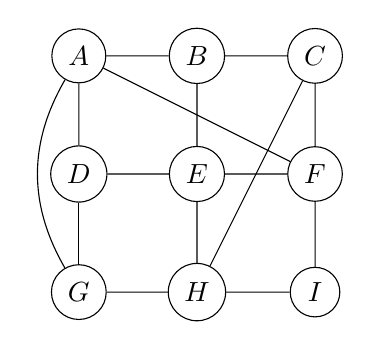
\begin{tikzpicture}[vert/.style={circle, draw}, scale=1.5]
  \node[vert] (A) at (0,2) {$A$};
\node[vert] (B) at (1,2) {$B$};
\node[vert] (C) at (2,2) {$C$};
\node[vert] (D) at (0,1) {$D$};
\node[vert] (E) at (1,1) {$E$};
\node[vert] (F) at (2,1) {$F$};
\node[vert] (G) at (0,0) {$G$};
\node[vert] (H) at (1,0) {$H$};
\node[vert] (I) at (2,0) {$I$};

\draw (A)--(B)--(C)--(F)--(A)--(D)--(E)--(F)--(I)--(H)--(G) to [bend left] (A);
\draw (D)--(G);
\draw (C)--(H)--(E)--(B);
\end{tikzpicture}
\end{center}
  \begin{block}{Give another proof that $\Gamma$ isn't planar}

    \end{block}


  \end{frame}


\end{document}
